\documentclass[a4paper]{article}

%% Language and font encodings
\usepackage{polski}
\usepackage[polish]{babel}
\usepackage[utf8x]{inputenc}
\usepackage[T1]{fontenc}
\usepackage{pdfpages}
\usepackage{indentfirst}
\usepackage{listings}

% Adjust penalties
\brokenpenalty=1000
\clubpenalty=1000
\widowpenalty=1000

%% Sets page size and margins
\usepackage[a4paper]{geometry}

%% Useful packages
\usepackage{amsmath}
\usepackage{graphicx}
\usepackage[colorlinks=true, allcolors=blue]{hyperref}
\usepackage{booktabs}

\usepackage{float}

\renewcommand\thesection{\arabic{section}.}
\renewcommand\thesubsection{\arabic{section}.\arabic{subsection}.}
\renewcommand\thesubsubsection{\arabic{section}.\arabic{subsection}.\arabic{subsubsection}.}

\title{Sprawozdanie nr 1}
\author{
Bartosz Jasiński \\
Adrian Sadłocha \\
Andrzej Wódkiewicz
}

\begin{document}
\maketitle
\setcounter{secnumdepth}{2}
\setcounter{tocdepth}{2}

\section{Prawo Ohma}

\subsection{Opis ćwiczenia}

Celem ćwiczenia było wyznaczenie rezystancji oporników $R_1$, $R_2$, $R_3$ oraz $R_4$.
Obwód był złożony z szeregowo podłączonego cyfrowego amperomierza, równolegle podłączonego analogowego woltomierza, rezystora oraz z zasilacza.

\subsection{Wstęp teoretyczny}

\subsubsection{Prawo Ohma}

Prądem nazywamy uporządkowany ruch ładunków elektrycznych.
W obwodzie elektrycznym stosunek napięcia do natężenia prądu jest stały:

$$\frac{U}{I} = \text{const}$$

Powyższa zależność jest nazywama \textit{prawem Ohma}. Powyższą stałą nazywamy rezystancją (oporem) i zwyczajowo oznaczamy za pomocą litery $R$.

\subsubsection{Niepewności pomiarowe}

Niepewnością pomiarową nazywamy miarę dokładności wykonanego pomiaru.
Wśród pomiarów bezpośrednich wyróżniamy dwa rodzaje metod wyliczania niepewności.

\begin{itemize}
\item Metody typu A -- jest to klasa metod, która oblicza niepewność za pomocą statystycznych technik badania analizy ciągu wyników pomiarów;
\item Metody typu B -- klasa metod, które opierają się na innych metod niż metody typu A, np. metody biorące pod uwagę własności przyrządów pomiarowych.
\end{itemize}

\subsection{Analiza wyników}

Pierwsze ćwiczenie służyło zbadaniu relacji między napięciem a natężeniem prądu.
W tym celu dokonaliśmy 10 pomiarów napięcia na rezystorze $R_4$ oraz 10 pomiarów natężenia prądu.
Uzyskane wyniki zostały przedstawione w tabeli oraz na wykresie zależności napięcia na $R_4$ od natężenia prądu.

Dla użytego woltomierza, przy zakresie $Z(U)$, niepewność wyznaczenia napięcia wynosi:

$$u_U = \frac{1\% \cdot Z(U)}{\sqrt{3}}$$

Niepewność wyznaczenia natężenia prądu (przy użytym amperomierzu) jest zależna od odczytanej wartości i wynosi:

$$u_I = \frac{1.2\% \text{rdg} + 1 \text{dgt}}{\sqrt{3}}$$

\begin{table}
\centering
\begin{tabular}{lrrrrrr}
\toprule
Lp. &  $U$ (V) &  $Z(U)$ (V) &  $u_U$ (V) &  $I$ (mA) &  $Z(I)$ (mA) &  $u_I$ (mA) \\
\midrule
1 &          8.80  &                10 &                 0.06  &             22.8  &                 200 &                     0.2 \\
2 &          8.00  &                10 &                 0.06  &             20.5  &                 200 &                     0.2 \\
3 &          7.00  &                10 &                 0.06  &             17.93 &                  20 &                     0.13 \\
4 &          6.20  &                10 &                 0.06  &             15.74 &                  20 &                     0.11 \\
5 &          5.20  &                10 &                 0.06  &             13.51 &                  20 &                     0.10 \\
6 &          4.40  &                10 &                 0.05  &             11.23 &                  20 &                     0.08 \\
7 &          3.60  &                10 &                 0.06  &              9.06 &                  20 &                     0.07 \\
8 &          2.600  &                 3 &                 0.018 &              6.76 &                  20 &                     0.05 \\
9 &          1.800  &                 3 &                 0.018 &              4.50 &                  20 &                     0.04 \\
10 &         0.86 &                 1 &                 0.01 &              2.29 &                  20 &                     0.02 \\
\bottomrule
\end{tabular}
\caption{Wielokrotne pomiary prądu $I_{R_4}$ i napięcia $U_{R_4}$ na rezystorze $R_4$.}
\end{table}

Na podstawie pomiarów napięcia i natężenia -- oraz uwzględniając błędy pomiarowe -- możemy stwierdzić, że natężenie prądu rośnie wprost proporcjonalnie do napięcia.
Stosunek napięcia do natężenia jest stały.
Wyniki doświadczenia potwierdzają słuszność prawa Ohma.

\subsection{Regresja liniowa}

Używając metody najmniejszych kwadratów można wyznaczyć współczynnik kierunkowy prostej $y = ax + b$.
Ponieważ napięcie i natężenie prądu są powiązane postacią $U = RI$, to przyjmujemy $b = 0$.
Zatem dopasowywana prosta będzie postaci $y = ax$.

Współczynnik kierunkowy szukanej prostej będzie szukaną rezystancją opornika. Ponadto, rezystancja ta będzie wyrażona wzorem:

$$a = \frac{\sum_{i = 1}^{10}\frac{I_i U_i}{u_{U_i}^2}}{\sum_{i = 1}^{10}\frac{I_i^2}{u_{U_i}^2}}$$

Z niepewnością wynoszącą:

$$u_a = \sqrt{\frac{1}{\sum_{i = 1}^{10}\frac{I_i^2}{u_{U_i}^2}}}$$

W celu wyznaczenia powyższych wartości pomocna będzie tabela z pośrednimi wartościami obliczeń.

\begin{table}
\centering
\begin{tabular}{lrrrrrrrrr}
\toprule
{} &     $U$ &       $u_U$ &      $I$ &       $u_I$ &       $IU$ &     $u_U^2$ &       $I^2$ &    $\frac{I^2}{u_U^2}$ & $\frac{IU}{u_U^2}$ \\
\midrule
0 &  8.80 &  0.057735 &  22.80 &  0.215698 &  200.6400 &  0.003333 &  519.8400 &  155952.00 &  60192.00 \\
1 &  8.00 &  0.057735 &  20.50 &  0.199763 &  164.0000 &  0.003333 &  420.2500 &  126075.00 &  49200.00 \\
2 &  7.00 &  0.057735 &  17.93 &  0.129996 &  125.5100 &  0.003333 &  321.4849 &   96445.47 &  37653.00 \\
3 &  6.20 &  0.057735 &  15.74 &  0.114823 &   97.5880 &  0.003333 &  247.7476 &   74324.28 &  29276.40 \\
4 &  5.20 &  0.057735 &  13.51 &  0.099374 &   70.2520 &  0.003333 &  182.5201 &   54756.03 &  21075.60 \\
5 &  4.40 &  0.057735 &  11.23 &  0.083577 &   49.4120 &  0.003333 &  126.1129 &   37833.87 &  14823.60 \\
6 &  3.60 &  0.057735 &   9.06 &  0.068543 &   32.6160 &  0.003333 &   82.0836 &   24625.08 &   9784.80 \\
7 &  2.60 &  0.017321 &   6.76 &  0.052608 &   17.5760 &  0.000300 &   45.6976 &  152325.33 &  58586.67 \\
8 &  1.80 &  0.017321 &   4.50 &  0.036950 &    8.1000 &  0.000300 &   20.2500 &   67500.00 &  27000.00 \\
9 &  0.86 &  0.005774 &   2.29 &  0.021639 &    1.9694 &  0.000033 &    5.2441 &  157323.00 &  59082.00 \\
\midrule
	suma & {} & {} & {} & {} & {} & {} & {} & 947160.06 & 366674.07 \\
\bottomrule
\end{tabular}
\caption{Wartości pośrednie obliczeń, które pozwalają wyznaczyć wartość współczynnika kierukowego w zagadnieniu regresji liniowej. Zachowaliśmy dodatkowe cyfry znaczące, aby uniknąć błędów numerycznych przy kolejnych obliczeniach.}
\end{table}

Otrzymujemy $a = \frac{366674.07}{947160.06} \approx 0.387$ oraz $u_a = \sqrt{\frac{1}{947160.06}} \approx 0.00101 \enskip \text{k}\Omega \approx 1.1 \enskip \Omega$.

Zatem opór $R_4 = 387.1 \, (1.1) \enskip \Omega$.

\begin{table}
\centering
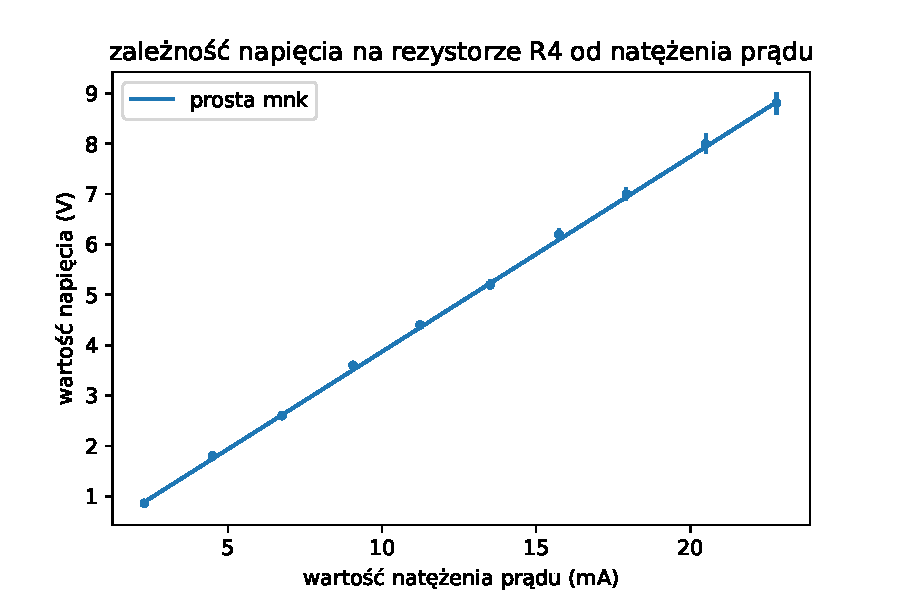
\includegraphics[scale=0.7]{fig_d.pdf}
\caption{Wyliczona prosta regresji liniowej zestawiona wraz ze zmierzonymi wartościami napięcia oraz natężenia prądu.}
\end{table}

\subsection{Obliczenia wartości $R_1$, $R_2$, $R_3$}

Niepewności napięcia oraz natężenie prądu są liczone jak wyżej.

Niepewność rezystancji wyznaczonej za pomocą wzoru $R = \frac{U}{I}$ wynosi:

$$u_R = \sqrt{(\frac{\partial R}{\partial U})^2 \cdot u_U^2 + (\frac{\partial R}{\partial I})^2 \cdot u_I^2} = \sqrt{\frac{1}{I^2} \cdot u_U + \frac{U^2}{I^2} \cdot u_I}$$

\begin{table}
\centering
\begin{tabular}{lrrrrrrl}
\toprule
Rezystor &  $U$ (V) &  $u_U$ (V) &  $I$ (mA) &  $u_I$ (mA) &  R ($\Omega$) &  $u_R$ ($\Omega$) \\
\midrule
$R_1$ &          2.85 &           0.018 &                  55.30 &              0.45 &             51.537 &             0.035 \\
$R_2$ &          4.0 &           0.06 &                  38.50 &              0.33 &            103.90 &             0.06 \\
$R_3$ &          4.0 &           0.06 &                  38.50 &              0.33 &            103.90 &             0.06 \\
\bottomrule
\end{tabular}
\caption{Wyniki pojedynczych pomiarów na rezystorach $R_1$, $R_2$ oraz $R_3$}
\end{table}

Zatem wartości $R_1$, $R_2$, $R_3$ wynoszą (zapis na trzy sposoby):

\begin{itemize}
\item $R_1 = 51.537 \enskip \Omega$, $u_{R_1} = 0.035 \enskip \Omega$
\item $R_2 = 103.90 \enskip \Omega$, $u_{R_2} = 0.06 \enskip \Omega$
\item $R_3 = 103.90 \enskip \Omega$, $u_{R_3} = 0.06 \enskip \Omega$
\end{itemize}

\begin{itemize}
\item $R_1 = 51.537 \, (35) \enskip \Omega$
\item $R_2 = 103.90 \, (6) \enskip \Omega$
\item $R_3 = 103.90 \, (6) \enskip \Omega$
\end{itemize}

\begin{itemize}
\item $R_1 = 51.537 \, (0.035) \enskip \Omega$
\item $R_2 = 103.90 \, (0.06) \enskip \Omega$
\item $R_3 = 103.90 \, (0.06) \enskip \Omega$
\end{itemize}

\section{Pomiary wielkości mechanicznych}

\subsection{Za pomocą suwmiarki}

Rozdzielczość suwmiarki wynosi $\Delta x = 0.02$ mm, zatem niepewność typu B wynosi: $u_B(x) = \frac{\Delta x}{\sqrt{3}} \approx 0.01154700 \approx 0.012$ mm.

Zatem wartości $l_1$, $l_2$, $l_3$ wynoszą (zapis na trzy sposoby):
Uzyskane pomiary trzech różncyh wielkości wyniosły kolejno: $36.60$ mm, $37.42$ mm, $30.70$.

\begin{itemize}
\item $l_1 = 36.600 \enskip \text{mm}$, $u_B = 0.012 \enskip \text{mm}$
\item $l_2 = 37.420 \enskip \text{mm}$, $u_B = 0.012 \enskip \text{mm}$
\item $l_3 = 30.700 \enskip \text{mm}$, $u_B = 0.012 \enskip \text{mm}$
\end{itemize}

\begin{itemize}
\item $l_1 = 36.600 \, (12) \enskip \text{mm}$
\item $l_2 = 37.420 \, (12) \enskip \text{mm}$
\item $l_3 = 30.700 \, (12) \enskip \text{mm}$
\end{itemize}

\begin{itemize}
\item $l_1 = 36.600 \, (0.012) \enskip \text{mm}$
\item $l_2 = 37.420 \, (0.012) \enskip \text{mm}$
\item $l_3 = 30.700 \, (0.012) \enskip \text{mm}$
\end{itemize}

\subsection{Wyniki pomiarów śrubą mikrometryczną}

W tym ćwiczeniu, za pomocą śruby mikrometrycznej, badana była grubość metalowej płytki.
Wykonane 60 pomiarów przedstawiliśmy w tabeli oraz za pomocą histogramu.

\begin{table}
\centering
\begin{tabular}{|l|l|l|l|l|l|}
\hline
2.94 & 2.93 & 2.94 & 2.92 & 2.94 & 2.95 \\
\hline
2.93 & 2.93 & 2.97 & 2.94 & 2.93 & 2.93 \\
\hline
2.93 & 2.94 & 2.93 & 2.93 & 2.94 & 2.93 \\
\hline
2.94 & 2.93 & 2.94 & 2.92 & 2.93 & 2.94 \\
\hline
2.93 & 2.94 & 2.94 & 2.93 & 2.94 & 2.94 \\
\hline
2.94 & 2.95 & 2.95 & 2.93 & 2.93 & 2.94 \\
\hline
2.94 & 2.93 & 2.94 & 2.94 & 2.94 & 2.93 \\
\hline
2.94 & 2.94 & 2.94 & 2.94 & 2.94 & 2.93 \\
\hline
2.94 & 2.93 & 2.93 & 2.94 & 2.93 & 2.94 \\
\hline
2.94 & 2.94 & 2.94 & 2.94 & 2.93 & 2.93 \\
\hline
\end{tabular}
\caption{Wyniki wielokrotnych pomiarów grubości płytki za pomocą śruby mikrometrycznej.}
\end{table}

\begin{table}
\centering
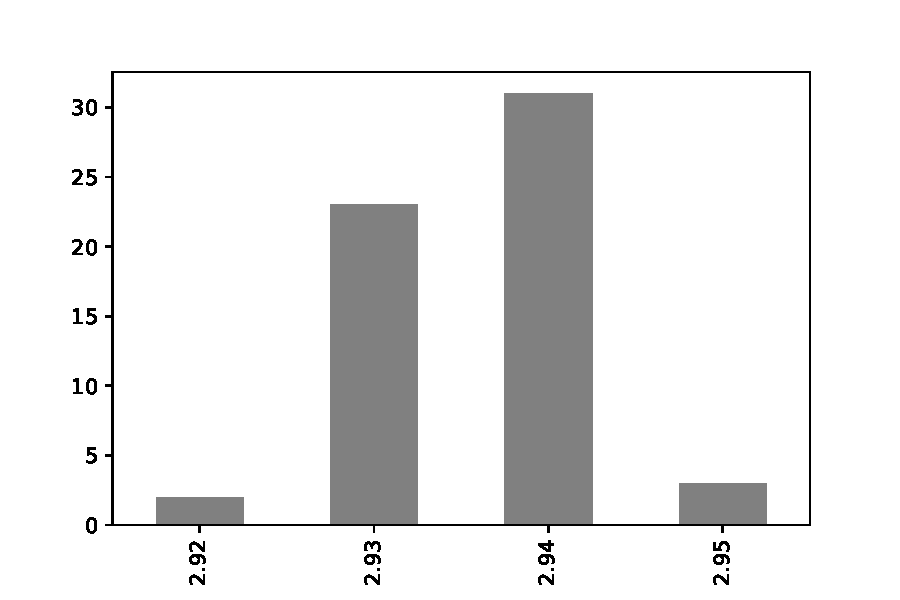
\includegraphics[scale=0.7]{hist.pdf}
\caption{Histogram pomiarów grubości płytki za pomocą śruby mikrometrycznej.}
\end{table}

Oznaczmy pomiary jako $x_i$, $i = 1, \dots, 60$.
Średnia wartość wszystkich pomiarów wynosi: $x = \frac{1}{60} \sum_{i = 1}^{60} x_i = \frac{1}{60} \cdot 176.19 = 2.9365$.
Odchylenie standardowe: $s_x = \sqrt{\frac{\sum_{i=1}^{60} (x_i - x)^2}{60 - 1}} \approx 0.0077733$.

Niepewność typu A: $u_x (\text{typ A}) = \frac{s_x}{\sqrt{60}} \approx 0.001004 \enskip \text{mm} \approx 0.0011 \enskip \text{mm}$.

Niepewność typu B: $u_x (\text{typ B}) = \sqrt{\frac{(\Delta x)^2}{3} + \frac{(\Delta x_e)^2}{3}} = \sqrt{\frac{(0.01)^2}{3} + \frac{(0.005)^2}{3}} \approx 0.006454972 \approx 0.0065 \enskip \text{mm}$.

Niepewność całkowita: $u_x = \sqrt{(u_x (\text{typ A}))^2 + (u_x (\text{typ B}))^2} \approx 0.00659242 \approx 0.0066$.

Ostatecznie, grubość płytki wynosi (zapis na 3 sposoby):

\begin{itemize}
\item $d = 2.9365$ mm, $u_x = 0.0066$ mm
\item $d = 2.9365 \, (66)$ mm
\item $d = 2.9365 \, (0.0066)$ mm
\end{itemize}

\subsection{Wyznaczanie objętości płytki}

Zmierzone zostały trzy wymiary metalowej płytki.
Oznaczmy objętość $V = x \cdot y \cdot z$, gdzie $x = 37.510 (0.012)$ mm, $y = 30.700 (0.012)$ mm, $z = 2.9365 (0.0066)$ mm.
Zauważmy, że $x$ oraz $y$ są obarczone niepewnościami typu B, zaś $z$ niepewnością typu A oraz B.
W celu wyznaczenia objętości $V$ wraz z niepewnością całkowitą, posłużymy się następującymi oznaczeniami oraz wzorami:

$$V = x \cdot y \cdot z = 37.510 \cdot 30.700 \cdot 2.9365 \enskip \text{mm}^3 = 3381.5471305 \enskip \text{mm}^3 \approx 3382 \enskip \text{mm}^3$$

\begin{align*}
u_V &= \sqrt{(\frac{\partial V}{\partial x})^2 \cdot u_x^2 + (\frac{\partial V}{\partial y})^2 \cdot u_y^2 + (\frac{\partial V}{\partial z})^2 \cdot (u_z \text{(typ A)})^2 + (\frac{\partial V}{\partial z})^2 \cdot (u_z \text{(typ B)})^2} \\
	&= \sqrt{(yz \cdot u_x)^2 + (xz \cdot u_y)^2 + (xy \cdot u_z \text{(typ A)})^2 + (xy \cdot u_z \text{(typ B)})^2} \\
	&= \sqrt{(30.7 \cdot 2.9365 \cdot 0.012)^2 + (37.51 \cdot 2.9365 \cdot 0.012)^2 + (37.51 \cdot 30.7 \cdot 0.0011))^2 + (37.51 \cdot 30.7 \cdot 0.0065)^2} \enskip \text{mm}^3\\
	&\approx 60.21 \enskip \text{mm}^3 \\
	&\approx 61 \enskip \text{mm}^3
\end{align*}

Ostatecznie, objętość płytki wynosi (zapis na 3 sposoby):

\begin{itemize}
\item $V = 3382 \enskip \text{mm}^3$, $u_V = 61 \enskip \text{mm}^3$
\item $V = 3382 \, (61) \enskip \text{mm}^3$
\item $V = 3382 \, (61) \enskip \text{mm}^3$
\end{itemize}

\end{document}
